\documentclass[12pt]{article}

% All that confusing stuff

\usepackage[T1]{fontenc}
\usepackage{mathptmx}
\usepackage{graphicx}
\usepackage{wrapfig}
\usepackage{tikz}
\usepackage{setspace}

\topmargin 0.0in
\setlength{\textwidth} {420pt}
\setlength{\textheight} {620pt} 
\setlength{\oddsidemargin} {20pt}
\setlength{\marginparwidth} {72in}

\usepackage{fancyhdr} 
\usepackage{url}

\usepackage{latexsym}
\usepackage{amsfonts}

% set it so that subsubsections have numbers and they
% are displayed in the TOC (maybe hard to read, might want to disable)

\setcounter{secnumdepth}{3}
\setcounter{tocdepth}{3}

% define widow protection

\def\widow#1{\vskip #1\vbadness10000\penalty-200\vskip-#1}

\clubpenalty=10000  % Don't allow orphans
\widowpenalty=10000 % Don't allow widows

% this should give me the ability to use some math symbols that 
% were available by default in standard latex (i.e. \Box)

\usepackage{latexsym}

% define a little section heading that doesn't go with any number

\def\littlesection#1{
\widow{2cm}
\vskip 0.5cm
\noindent{\bf #1}
\vskip 0.0001cm 
}

\pagestyle{fancyplain}

\newcommand{\tstamp}{\today}   
\renewcommand{\sectionmark}[1]{\markright{#1}}
\lhead[\Section \thesection]            {\fancyplain{}{\rightmark}}
\chead[\fancyplain{}{}]                 {\fancyplain{}{}}
\rhead[\fancyplain{}{\rightmark}]       {\fancyplain{}{\thepage}}
\cfoot[\fancyplain{\thepage}{}]         {\fancyplain{\thepage}{}}

\newlength{\myVSpace}% the height of the box
\setlength{\myVSpace}{1ex}% the default, 
\newcommand\xstrut{\raisebox{-.5\myVSpace}% symmetric behaviour, 
  {\rule{0pt}{\myVSpace}}%
}

% leave things with no spacing extra spacing in the final version of the paper
\renewcommand{\baselinestretch}{1.0}    % must go before the begin of doc

% suppress the use of indentation for a paragraph

\setlength{\parindent}{0.0in}
\setlength{\parskip}{0.1in}

\begin{document}

% handle widows appropriately
\def\widow#1{\vskip #1\vbadness10000\penalty-200\vskip-#1}

% build the title section

\makeatletter

\def\maketitle{%
  %\null
  \thispagestyle{empty}%
  %\vfill
  \begin{center}%\leavevmode
    %\normalfont
    {\Huge \@title\par}%
    %\hrulefill\par
    {\normalsize \@author\par}%
    \vskip .4in
%    {\Large \@date\par}%
  \end{center}%
  %\vfill
  %\null
  %\cleardoublepage

  }

\makeatother


\vspace*{-1.1in}
\title{Flight Using Sensor Feedback}

% build the author section
\author{Cory Matthew Jones\\
Department of Computer Science\\
Allegheny College \\
{\tt jonesc@allegheny.edu}  \\
\vspace*{.1in} \today}

\vspace*{.1in} 

% use the default title stuff
\maketitle

	\begin{center} 
	  {\bf Abstract} 
	\end{center}

	\vspace*{-.1in} 
     
     My proposal is to program a model airplane to  navigate to a sequence GPS points, and capture infrared images of the ground at those designated points. The purpose of this work is to create a UAV that can take accurate  pictures of the land scape in infrared to allow gathering data about plants in the area. 
     
     %successfully fly on its own.  I will try to make a program that will utilize a total of four sensors to control the airplane. The program that I make should 
     
     %Creating a robot that works the way you intended it to is very difficult.  A robot can only preform explicitly what it is told to do.   No matter how sophisticated the robot, it will never have the common since that humans possess.    Without sensors robots have no way to interface with the physical world, Sensors give robots information that can actively be used to help it navigate through it's environment.  Robots use interpreted data from the sensors to decide what preprogrammed actions to take to navigate the environment, this can be called feedback control.  
     

\doublespacing

\vspace*{-.2in}
\section{Introduction}
\label{sec:Introduction}
\vspace*{-.1in}

  During the summer of 2011 two Allegheny College students, Ian Armstrong~(2012), and Anthony Smith built a programmable airplane.  In order for the plane to run they needed to install a motor and sensors.  Additionally, they needed a small programable computer to control the airplane.  By the end of their summer, they successfully built and programed the airplane to fly in a straight  line.  
  %However, only the gyroscope and accelerometer were successfully implemented.
  \\
  
  
  
  %paragraph about the Arduino and Ardupilot
  
  
  		%put this some where
  		%As a safety precaution the plane will feature a separate processor that will over ride the programming to allow for  manual control
  		
  		An Arduino is a small affordable device that can be bought from http://Arduino.cc/EN/.  The Arduino allows for average end-users to experiment with robotics the Arduino is “intended for artists, designers, hobbyists, and anyone interested in creating interactive objects or environments”.  The Arduino board is set up in such a way that users can use both digital and analog inputs in order for the Arduino to sense its environment.  During this project we plan to use a programming language called Occam-Pi.  Occam-Pi is a process oriented programming language.  This type of programming language focuses on processes.  However, Occam-Pi is not a native language on the Arduino so we have to install it on top of the existing language that is already on the Arduino.  
  		
  	\begin{figure}[htb]
	\begin{center}
	\leavevmode
	\vspace*{.5in}
	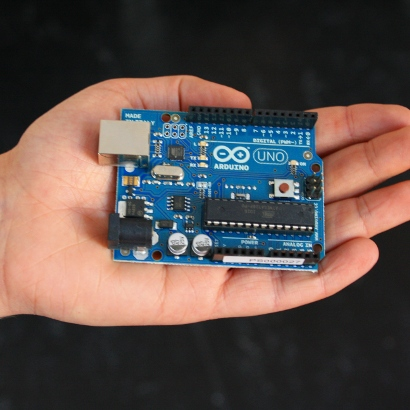
\includegraphics[width=100mm]{Arduino.jpg}
	\vspace*{.5in}
	\end{center}
	\caption{An Arduino \cite{Arduino.cc}}
	\label{fig:Arduino}
	\end{figure}
  		
  		
  		For the purposes of my project we will be using what an Ardupilot.
  		
  		
  	\begin{figure}[htb]
	\begin{center}
	\leavevmode
	\vspace*{.5in}
	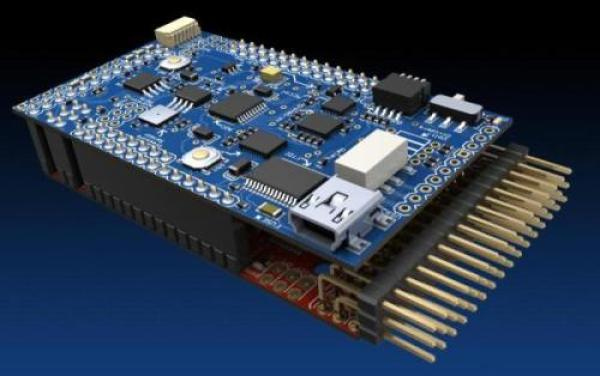
\includegraphics[width=100mm]{Ardupilot.jpg}
	\vspace*{.5in}
	\end{center}
	\caption{The Ardupilot \cite{diydrones}}
	\label{fig:Ardupilot}
	\end{figure}
  
  %paragraph about gyroscopes 
Gyroscope sensors are widely used in order to to interpret the orientation of a divice.  There are many different types of gyroscope sensors such as rotary gyroscopes, vibrating structure gyroscopes and optical gyroscopes.

\begin{figure}[htb]
\begin{center}
\leavevmode
\vspace*{.5in}
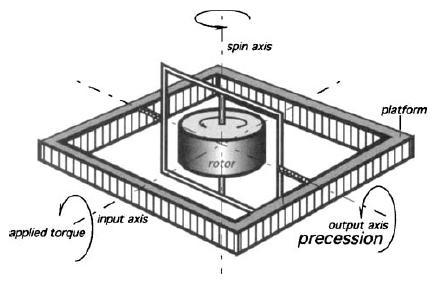
\includegraphics[width=100mm]{gyroscope_axes_crop.jpg}
\vspace*{.5in}
\end{center}
\caption{Rotary Gyroscope sensor \cite{Gyro}}
\label{fig:gyroR}
\end{figure}

Throughout all the different types of gyroscopes they all have at least one axis of measurements.  Recently with acceleration of technology gyroscopes can now have up to  3 axis on a single gyroscope.  3 axis gyroscopes combined with 3 axis accelerometers "provide a full 6 degrees of freedom (DoF) motion tracking system \cite{Gyro}~".


  %paragraph about accelerometers 
  
  %paragraph about wind speed measurer(pito tube)
  
  %paragraph about GPS
  
  %maybe a paragraph about Occam~-~∏
  
  Occam-~$\Pi$
  
  

  Currently the plane can fly in a straight line using only the gyroscope and accelerometer.  However, the airplane has yet to execute a turn without .  In part, this is because turns require a certain airspeed in order to execute successfully.  This is a major challenge in programming an airplane because the accelerometer becomes easily confused due to multiple forces such as gravity and other G forces pulling in different directions.  The conflicting sensor data is hard to interpret because the accelerometer reports the amount of force that it is pulled in. ****fill in more about why this matters****d
  
  Implementing a wind speed sensor will enable the plane to measure its speed while turning.  The plane can use the information to keep the proper air speed to stay aloft while turning.  The second sensor is the GPS which has a two and a half meeter resolution.  This means that the GPS sensor will accurately pin point the planes position within a imaginary bubble two and a half meeter's wide.  

\begin{figure}[htb]
\begin{center}
\leavevmode
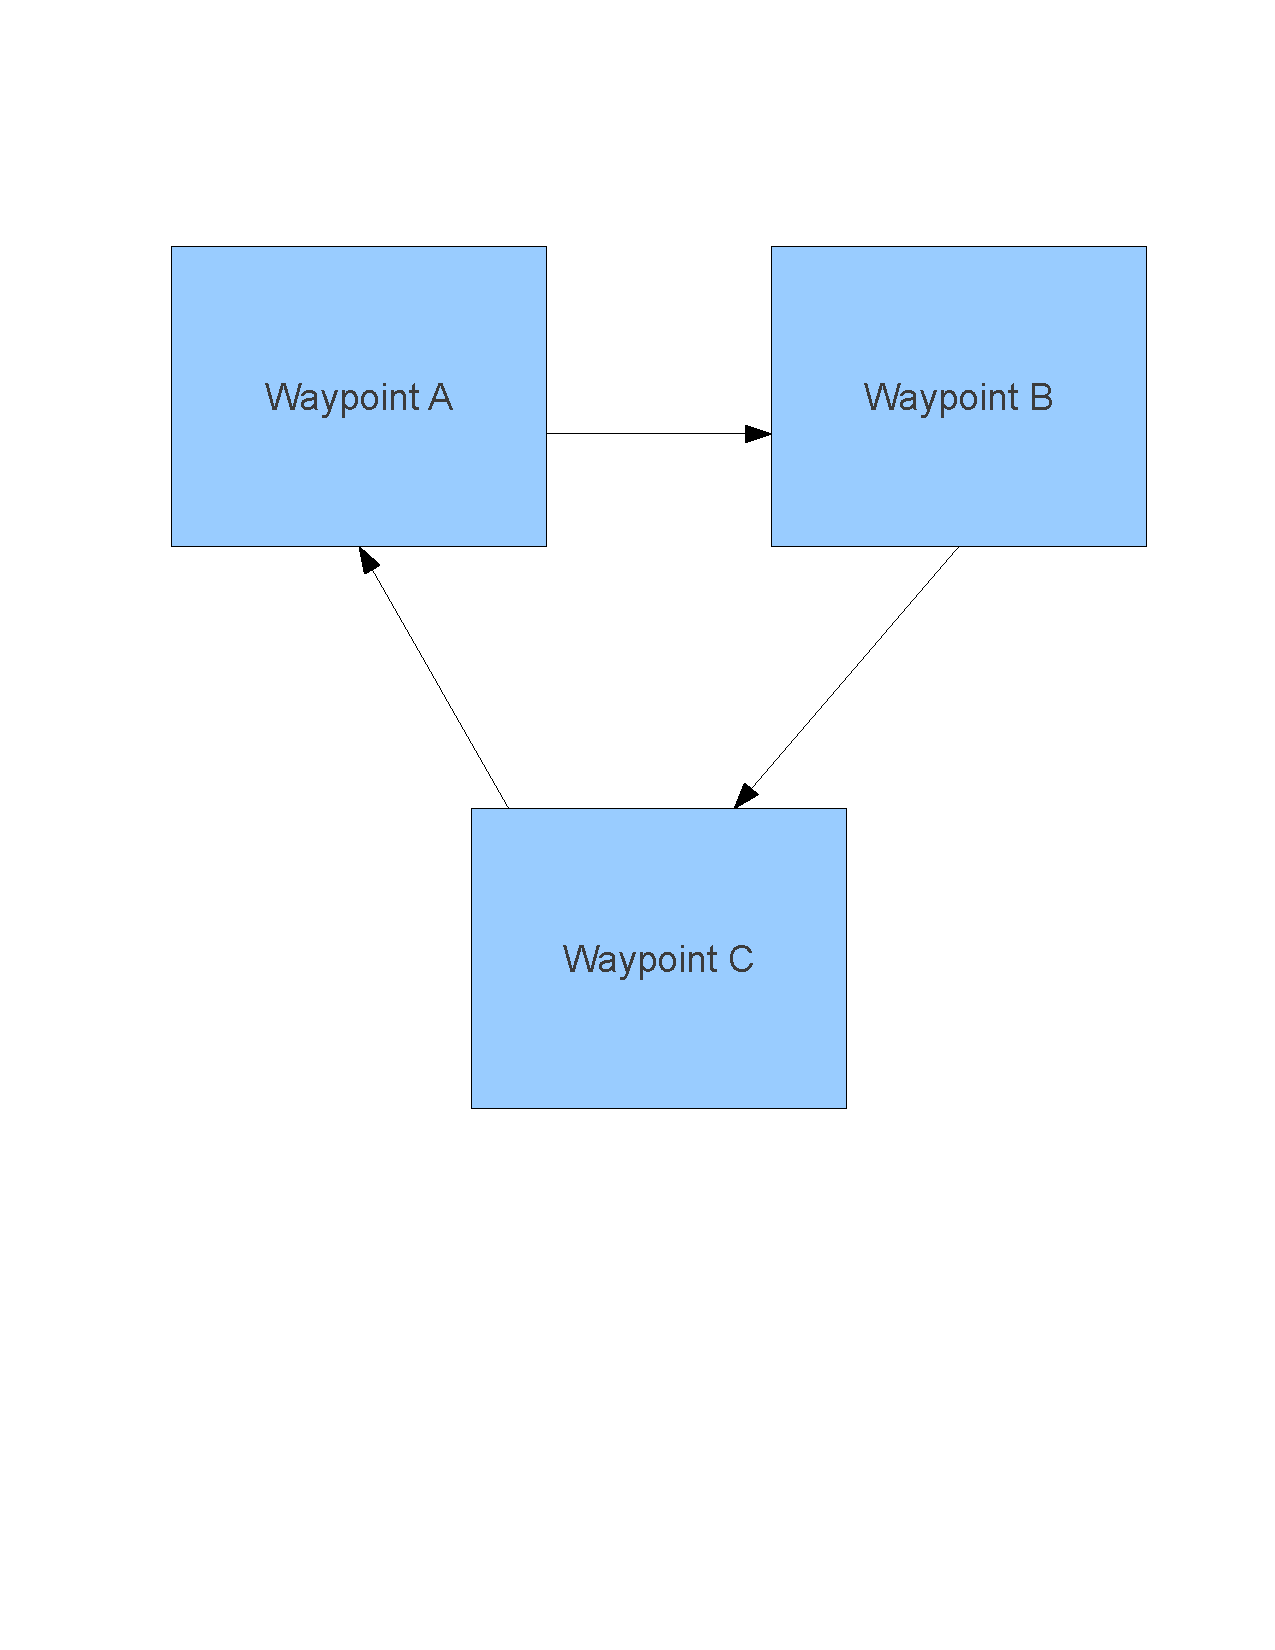
\includegraphics[width=100mm]{waypoints.pdf}
\vspace*{-1.5in}
\end{center}
\caption{Flying Waypoints}
\label{fig:Waypoints}
\end{figure}

Figure \ref{fig:Waypoints} shows a simple directional pattern that the airplane would follow.  There are many uses that way point flying plane could be used for.

\begin{figure}[htb]
\begin{center}
\leavevmode
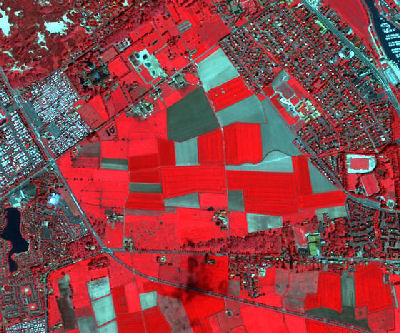
\includegraphics[width=100mm]{InfaPic}
\end{center}
\caption{Inferred Crop Imaging \cite{InfaPic}}
\label{fig:CropImg}
\end{figure} 

***this paragraph should make clear to the reader what we do and why it is valuable***\\
\newline
By completing an airplane that can reliably get from point A, to B, to C, many possibilities become practical.  Figure~\ref{fig:CropImg} shows a infrared picture taken by a satellite in 2005~\cite{InfaPic}.  I hope to successfully program the plane to turn successfully, and be able to travel to select way points.


%\vspace*{-.4in}
\section{Background}
\label{sec:Background}
\vspace*{-.1in}



A robot can perform many tasks, but those tasks must be preprogrammed.  
Different physical architectures give robots the ability to change what tasks 
are physically possible.  In addition, the architecture of a robot can affect 
how well a robot can preform specific tasks.  Essentially, a robot is a device 
that uses sensor information to preform specified actions given that certain 
programmed circumstances are met.  

\vspace*{-.1in}
\subsection{Sensors}
\label{sec:Sensors}
\vspace*{-.1in}


In order for any robot to function to a particular degree of accuracy, it must 
have sensors.  Without sensor feedback, a robot could be thought of as being  blind, as a result of no data being available to navigate its 
environment.  In general there are many different type of sensors, each type of 
sensor has its own uses and weaknesses.  The sensors that will be used in this 
proposal will fall into categories such as distance, speed, and location.

In order to fully utilize sensors, the programmer must have knowledge of how 
those sensors work.  For example, the Braitenberg Vehicle is a simple way of 
conveying fundamental information about the light sensor.  
\vspace*{.2in}  
\begin{figure}[htb]
\begin{center}
\leavevmode
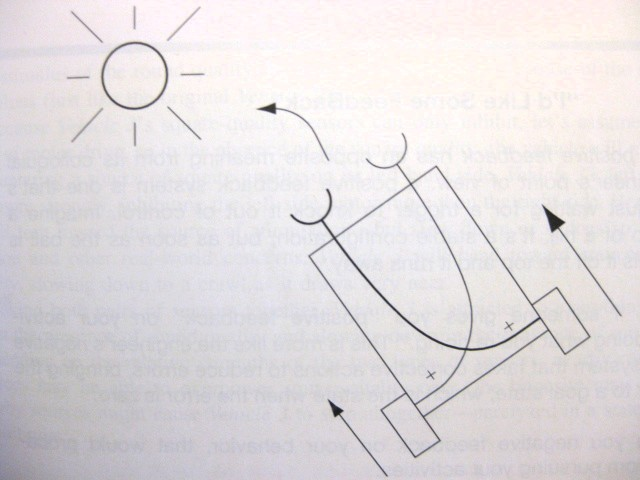
\includegraphics[width=100mm]{IMG_0003.JPG}
\end{center}
\caption{Braitenberg's Light Finder~\cite{RoboticExplorations} }
\label{fig:LightFinder}
\end{figure}

This vehicles basic function is to move towards the brightest spot it can find. 
In Figure~\ref{fig:LightFinder} each of the wires from the light sensors attach 
to a motor on the opposite side of the robot.  Lets assume that the larger the 
feedback value from the light sensor, the faster the motor linked to it will 
run. At first the wiring may seem contradictory to the robots goal.  However,  
think about the leftmost sensor.  The greater the feedback value, the greater 
the signal output, which in turn causes that motor to run faster.  So suppose 
that in this case the light value is stronger in the left most sensor.  This 
will cause the right motor to increase its speed proportionately to the light 
feedback value.  Remember,  the right most sensor is not receiving as strong of 
a light value from the sensor.  This will cause the left motor to run, but it 
will not run as fast as the right motor.  Due to the difference in speed between 
the motors, the robot will turn left towards the stronger light source.  
Overall, using a single sensor to preform actions is relatively simple.  
However, using multiple types of sensors used in conjunction can make this much 
more complicated.\\




    




\vspace*{-.2in}
\section{Evaluation Strategy}
\label{sec:evaluate}
\vspace*{-.1in}

Logically, some parts of evaluating whether or not the project works will be clear~(such as if the airplane fell out of the sky during a turn).  The most challenging part is ensuring that the GPS navigation works correctly every time.  For crop imaging to be successful, we must be able to take a picture of the same location reliably.  It is a given that our accuracy has a limit due to the resolution of the GPS sensor.  However,  giving leeway for that limit we can compare dozens of photos and see how accurately they match up.  This will allow us to evaluate the effectiveness of our airplanes  ability to follow and  take pictures of a preset path.  

\vspace*{-.1in}get
\section{Research Schedule}
\label{sec:schedule}
\vspace*{-.1in}

\begin{itemize}
\item 1 week to research how the gps works
\item 2-3 weeks test and build general direction based routing algorithm
\item 1 weekend to test gps and pitot tube walking.
\item 1 weekend to test gps and pitot tube while in car.
\item 1 weekend to capture raw data during remote control flight of plain.
\item 4-7 weeks program plane and test.
\item 2 weeks write proposal.
\item{
\textbf{Future Work:} Implement the third dimension axis.
}
\end{itemize}

\vspace*{-.1in}
\section{Conclusion}
\label{sec:conclusion}
\vspace*{-.1in}

Auto-piloted model planes are uncommon, and exceedingly expensive.  Creating a simple plain that can fly to pre-selected destinations can have many uses.  Crop imaging is a prime area in which work is being done.  However, taking pictures of the same place is too costly and expensive to implement long term.  The creation of this airplane will give experience to the programmer and allow for future work to evolve the usability of the system.  

\begin{singlespace}
\newpage
\bibliographystyle{plain}
\bibliography{senior_thesis_proposal_enhanced}

\end{singlespace}

\end{document}

